\documentclass[14pt, a4paper]{report}
\usepackage{mathtext}
\usepackage[T2A]{fontenc}
\usepackage[utf8]{inputenc}
\usepackage[russian]{babel}
\usepackage{multirow}
\usepackage{slashbox}
\usepackage{makecell}
\usepackage{graphicx}
\usepackage{physics}
\usepackage{amstext}
\usepackage{caption}
\usepackage{subcaption}
\usepackage{cmap}
\usepackage{float}
\usepackage{indentfirst}

\renewcommand{\thesection}{\arabic{section}.}
\renewcommand{\thesubsection}{\arabic{section}.\arabic{subsection}.}

\title{\textbf{Отчет о выполнении лабораторной работы 4.2 "Исследование энергетического спектра $\beta$-частиц и определение их максимальной энергии при помощи магнитного спектрометра"}}
\author{Калашников Михаил, Б03-202б}
\date{}

\begin{document}
\maketitle

\textbf{Цель работы:}
Исследовать с помощью магнитного спектрометра энергетический спектр $\beta$-частиц при распаде ядер $^{137}$Cs и определить их максимальную энергию. Откалибровать спектрометр по энергии электронов внутренней конверсии $^{137}$Cs.
\newline

\textbf{В работе используются:}
\begin{itemize}
\item цезиевый источник $\beta$-частиц;
\item магнитный спектрометр;
\item форвакуумный насос;
\item счетчик, подключенный к компьютеру;
\item выпрямитель сигналов.
\end{itemize}

\section{Теоретические сведения}

Бета-распадом называется самопроизвольное превращение ядер, при котором их массовое число остается прежним, а заряд изменяется на единицу. Бета-активные ядра встречаются во всей области значений массового числа A.
В данной работе будет изучен электронный распад
\[^A_Z X \rightarrow _{Z+1}^A X+e^-+\tilde{\nu},\]
при котором кроме электрона испускается антинейтрино.

Спектр энергии $\beta$-частиц оценивается формулой
\[\frac{dN}{dE}\approx\sqrt{E}(E_e-E)^2,\]
где $E_e$ -- максимальная энергия электронов.

Дочерние ядра, возникающие в результате $\beta$-распада, нередко оказываются возбужденными. Такие ядра отдают свою энергию либо излучая $\gamma$-квант, либо передевая избыток энергии одному из электронов с внутренних оболочек атома. Излучаемые в таком процессе электроны имеют строго определенную энергию и называются конверсионными.

\begin{figure}[H]
\centering
\makebox[\textwidth][c]{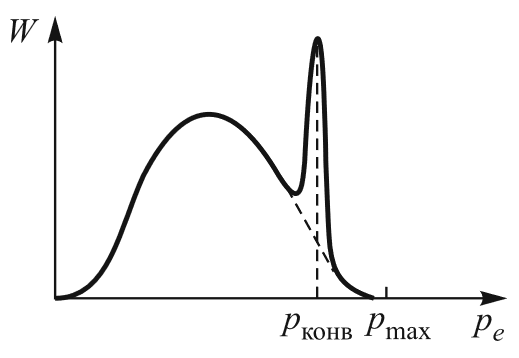
\includegraphics[scale=0.6]{../images/542-5}}
\caption{Форма спектра $\beta$-частиц}
\end{figure}

\section{Экспериментальная установка}

Для определения энергии $\beta$-частиц используется магнитный $\beta$-спектрометр. Электроны, испускаемые радиоактивным источником попадают в магнитное поле катушки. Траектории электронов в магнитном поле являются сложной спиралью, сходящимися в фокусе. В фокусе установлен детектор электронов.

Для заряженных частиц тонкая катушка эквивалентна линзе. Ее фокусное расстояние зависит от импульса электронов и от силы тока, протекающего через катушку.

\[\frac{1}{f}\propto\frac{I^2}{p_e^2}\]

Так как геометрия прибора в ходе эксперимента остается неизменной, то импульс сфокусированных электронов пропорционален величине тока:

\[p_e=kI.\]

Константу прибора можно определить сравнивая измеренное положение конверсионного пика с табличным значением.

\section{Проведение эксперимента}

\begin{enumerate}

\item Включим пересчетный прибор, высоковольтный выпрямитель и форвакуумный насос.

\item Дождемся откачки камеры спектрометра. Степень откачки будем измерять проводя измерения интенсивности $\beta$-излучения и отмечая уровень изменения показаний.

\item Приступим к измерению спектра. Будем повышать ток в катушке от 0 до 4.2 А с шагом 0.2 А. Каждое измерение длится 100 секунд. Получим следующий набор точек.

\item Из полученных измерений можно сделать вывод что конверсионный пик лежит в диапазоне от 3 до 3.6 А. Проведем измерения данного участка с шагом 0.05 А. Из всех точек вычтем среднее значение первой и последней точек, приняв его за фоновое излучение ($N_{ф}=(0.92\pm0.15)\ с^{-1}$).

\begin{figure}[H]
\centering
\makebox[\textwidth][c]{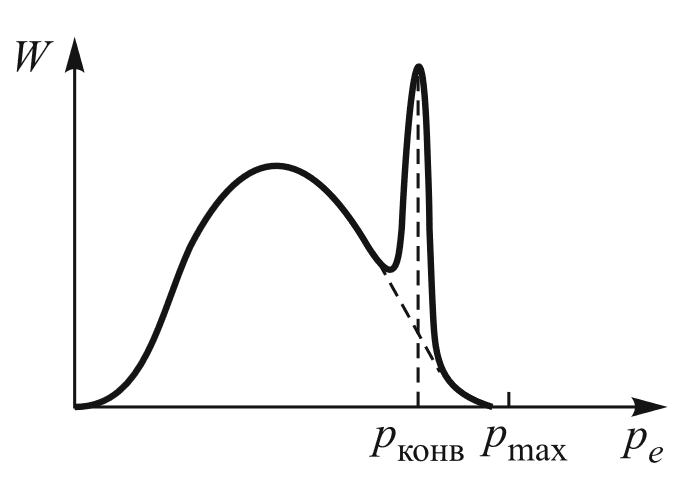
\includegraphics[scale=0.75]{../images/542-1}}
\caption{Первичное измерение спектра}
\end{figure}

\begin{figure}[H]
\centering
\makebox[\textwidth][c]{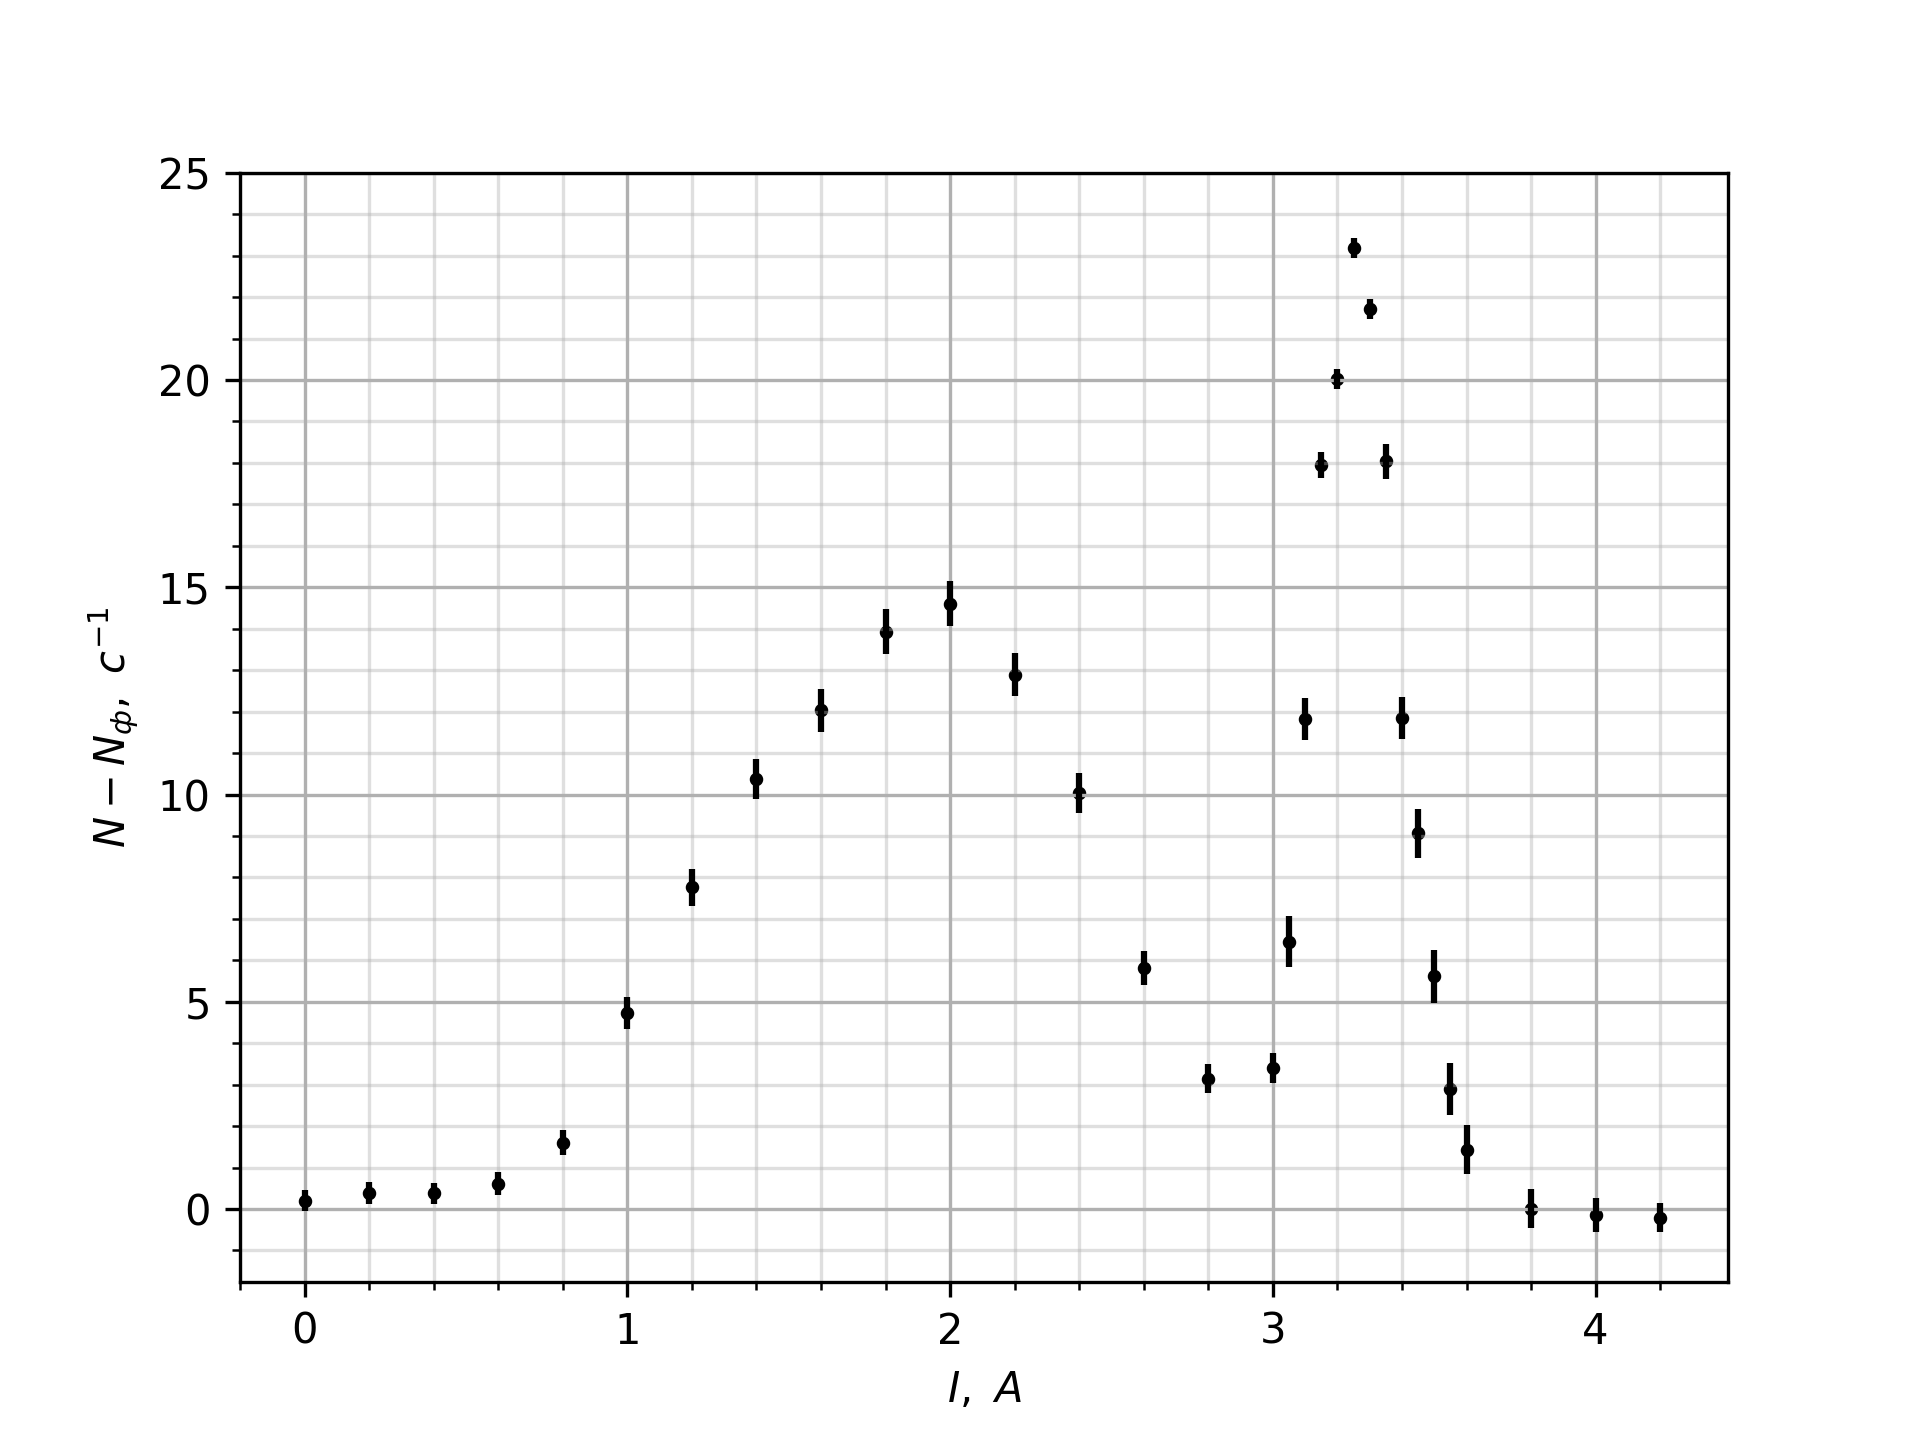
\includegraphics[scale=0.75]{../images/542-2}}
\caption{Измереный спектр $\beta$-излучения}
\end{figure}

\end{enumerate}

\section{Обработка результатов}

\begin{enumerate}

\item Проведем калибровку спектрометра. Для определения точного положения центра конверсионного пика аппроксимируем его гауссовой кривой:

\[N-N_{ф}=ae^{-\frac{(I-b)^2}{2c^2}}\]

Получим параметры:

\[a=(22.8\pm0.3)\ с^{-1},\quad b=(3.257\pm0.004)\ А,\quad c=(0.136\pm0.003)\ А\]

Следовательно, положение центра конверсионного пика:

\[I_{конв}=b=(3.257\pm0.004)\ А\]

\begin{figure}[H]
\centering
\makebox[\textwidth][c]{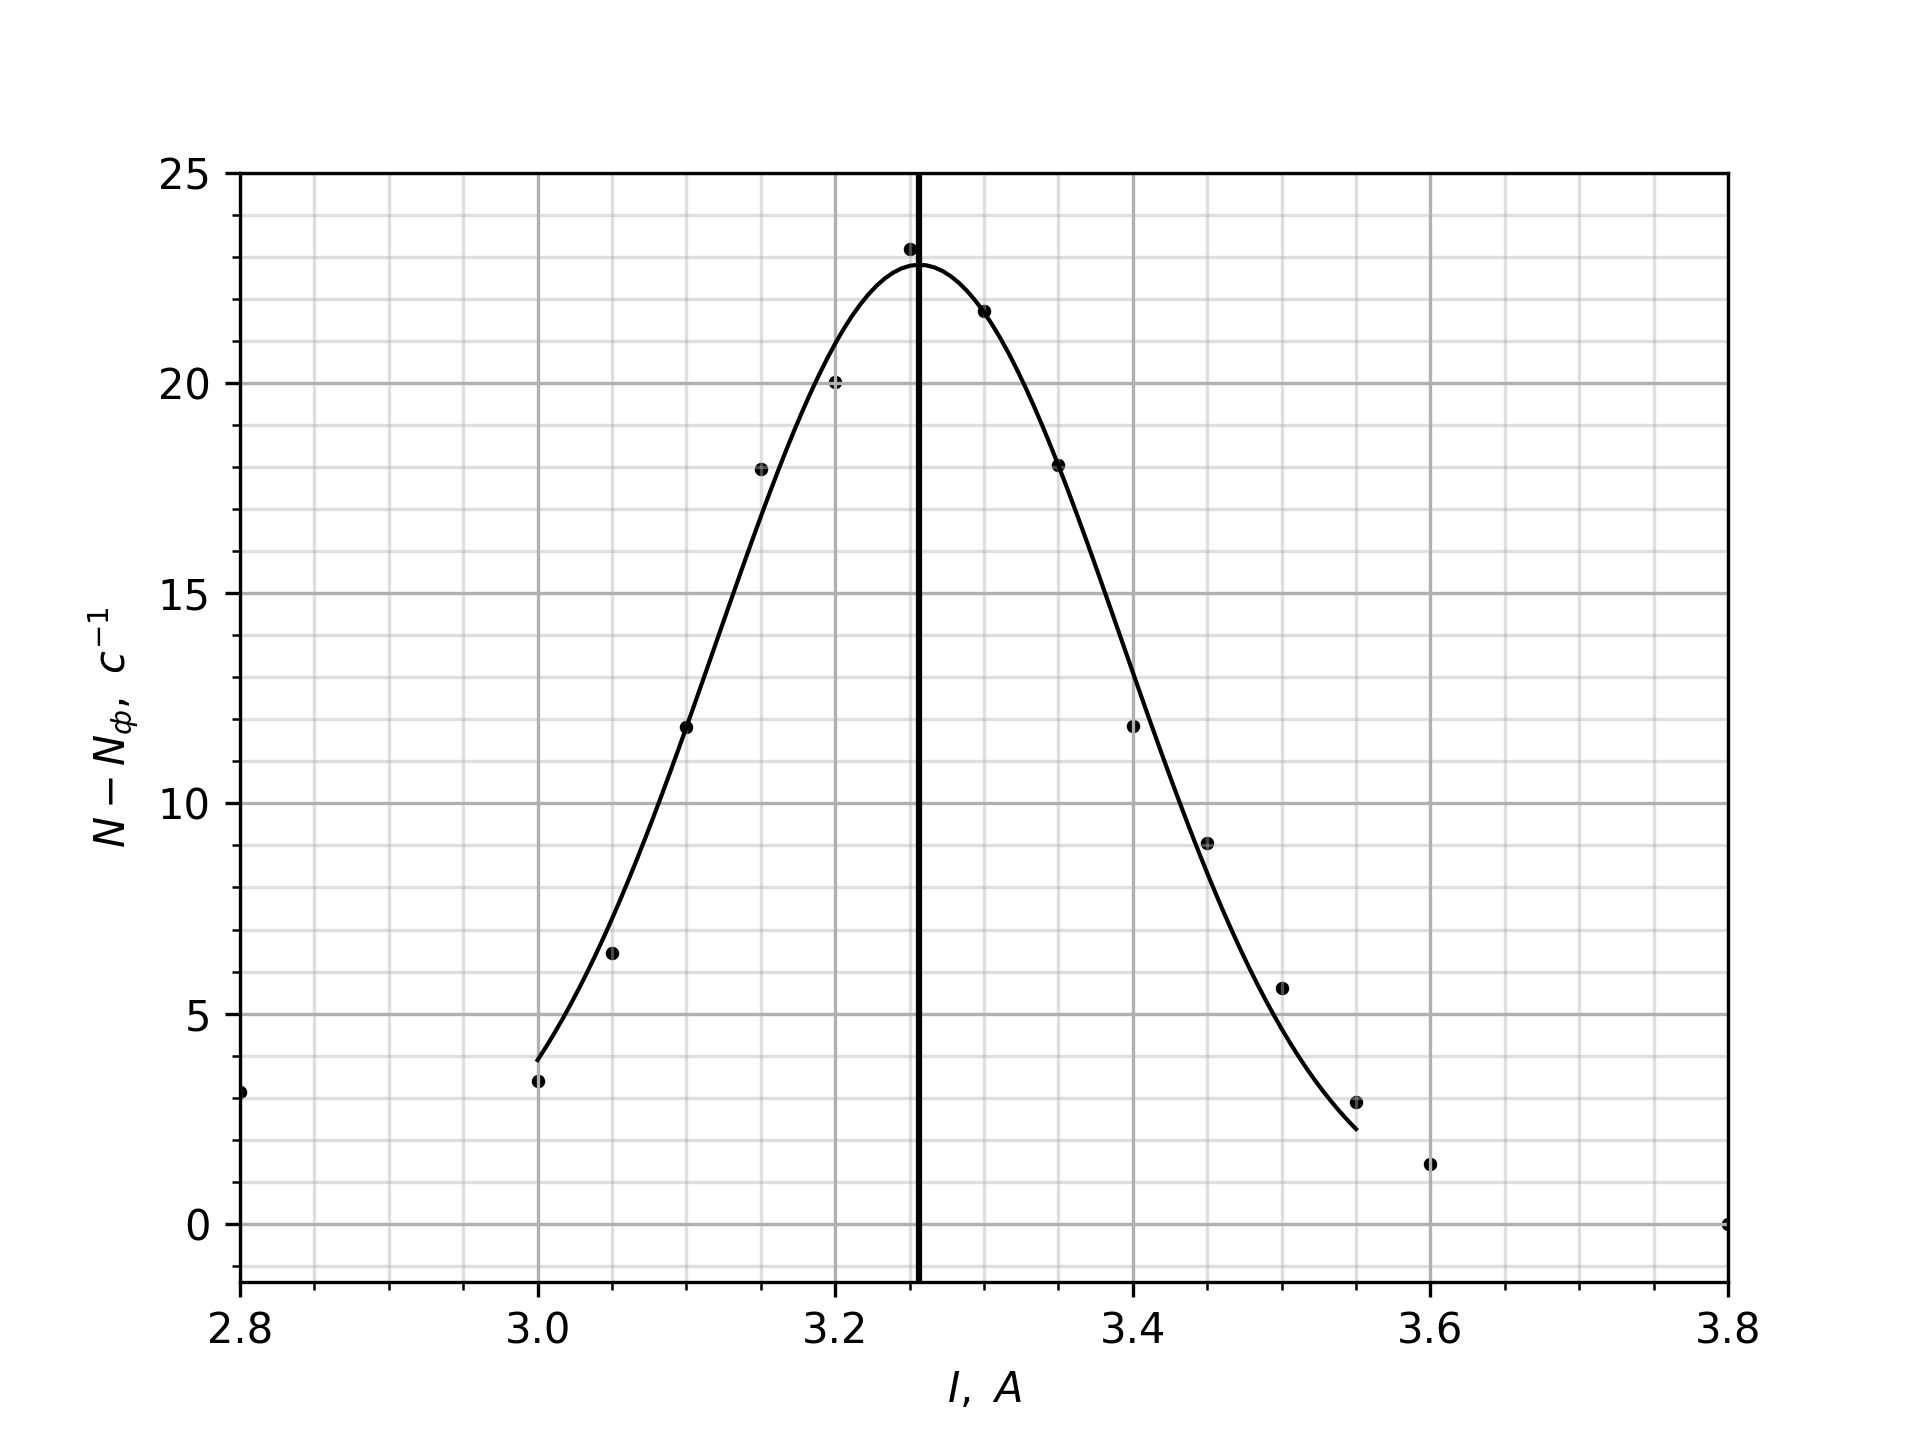
\includegraphics[scale=0.75]{../images/542-4}}
\caption{Аппроксимация конверсионного пика}
\end{figure}

\item Зная, что $(pc)_{конв}=1013.5\ кэВ$, рассчитаем константу прибора:

\[k=\frac{(pc)_{конв}}{I_{конв}}=(311.2\pm0.3)\ \frac{кэВ}{А}\]

Построим полученный спектр с тремя осями абсцисс -- сила тока, импульс и кинетическая энергия.

\begin{figure}[H]
\centering
\makebox[\textwidth][c]{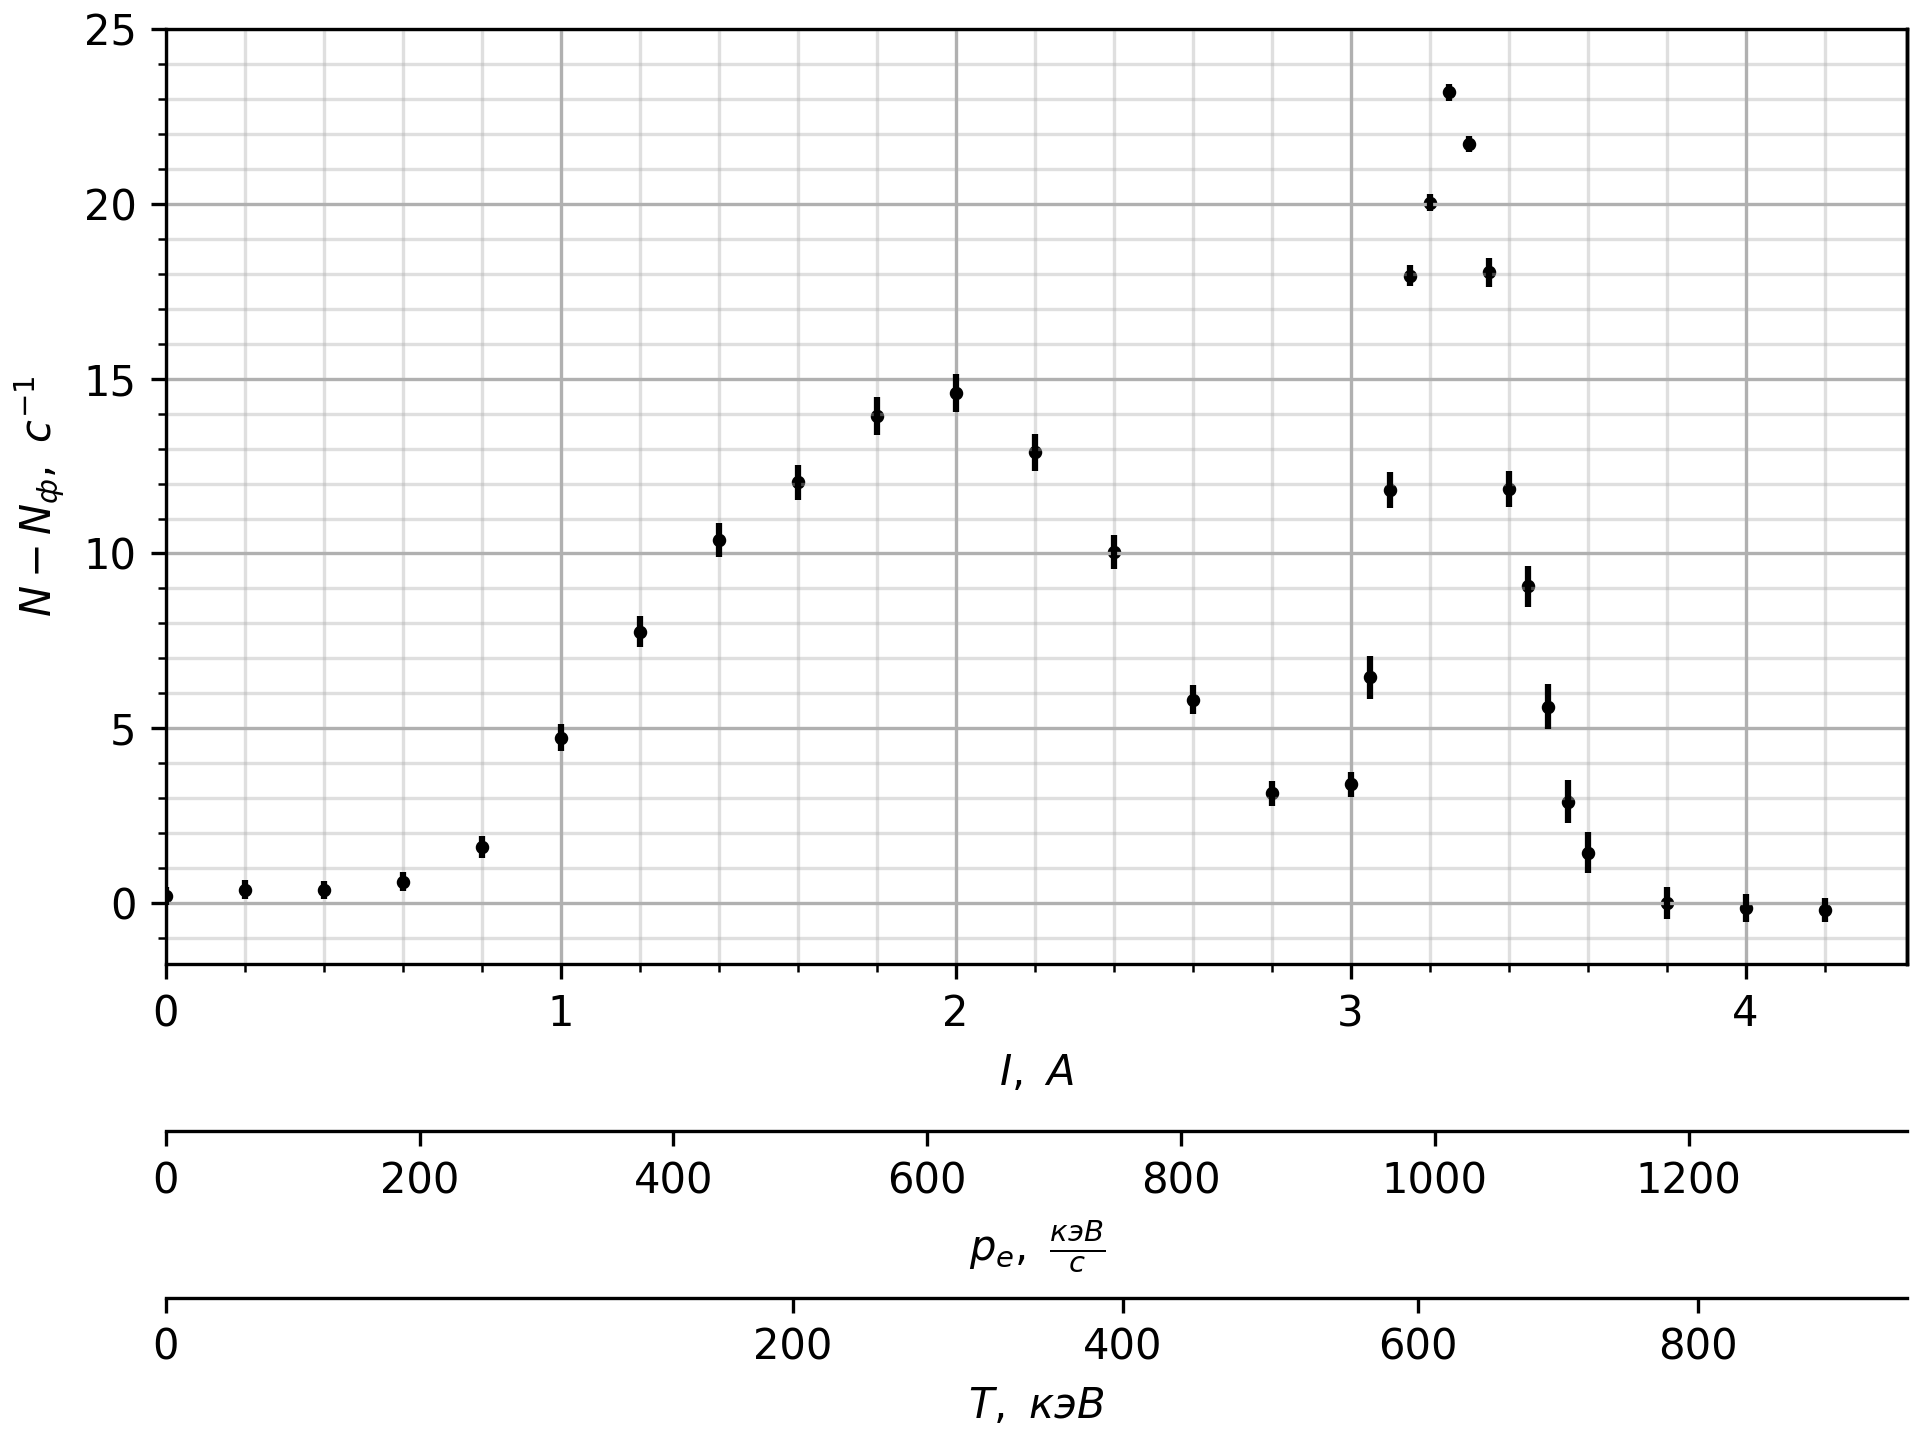
\includegraphics[scale=0.75]{../images/542-6}}
\caption{Измереный спектр $\beta$-излучения с дополнительными осями}
\end{figure}

\item Теперь можем построить график Ферми. Зная, что спектр описывается формулой

\[\sqrt{\frac{N-N_{ф}}{p^3}}=a(T_{max}-T),\]

построим график в координатах $\sqrt{(N-N_{ф})/p^3}$ по оси ординат и $T$ по оси абсцисс.

\begin{figure}[H]
\centering
\makebox[\textwidth][c]{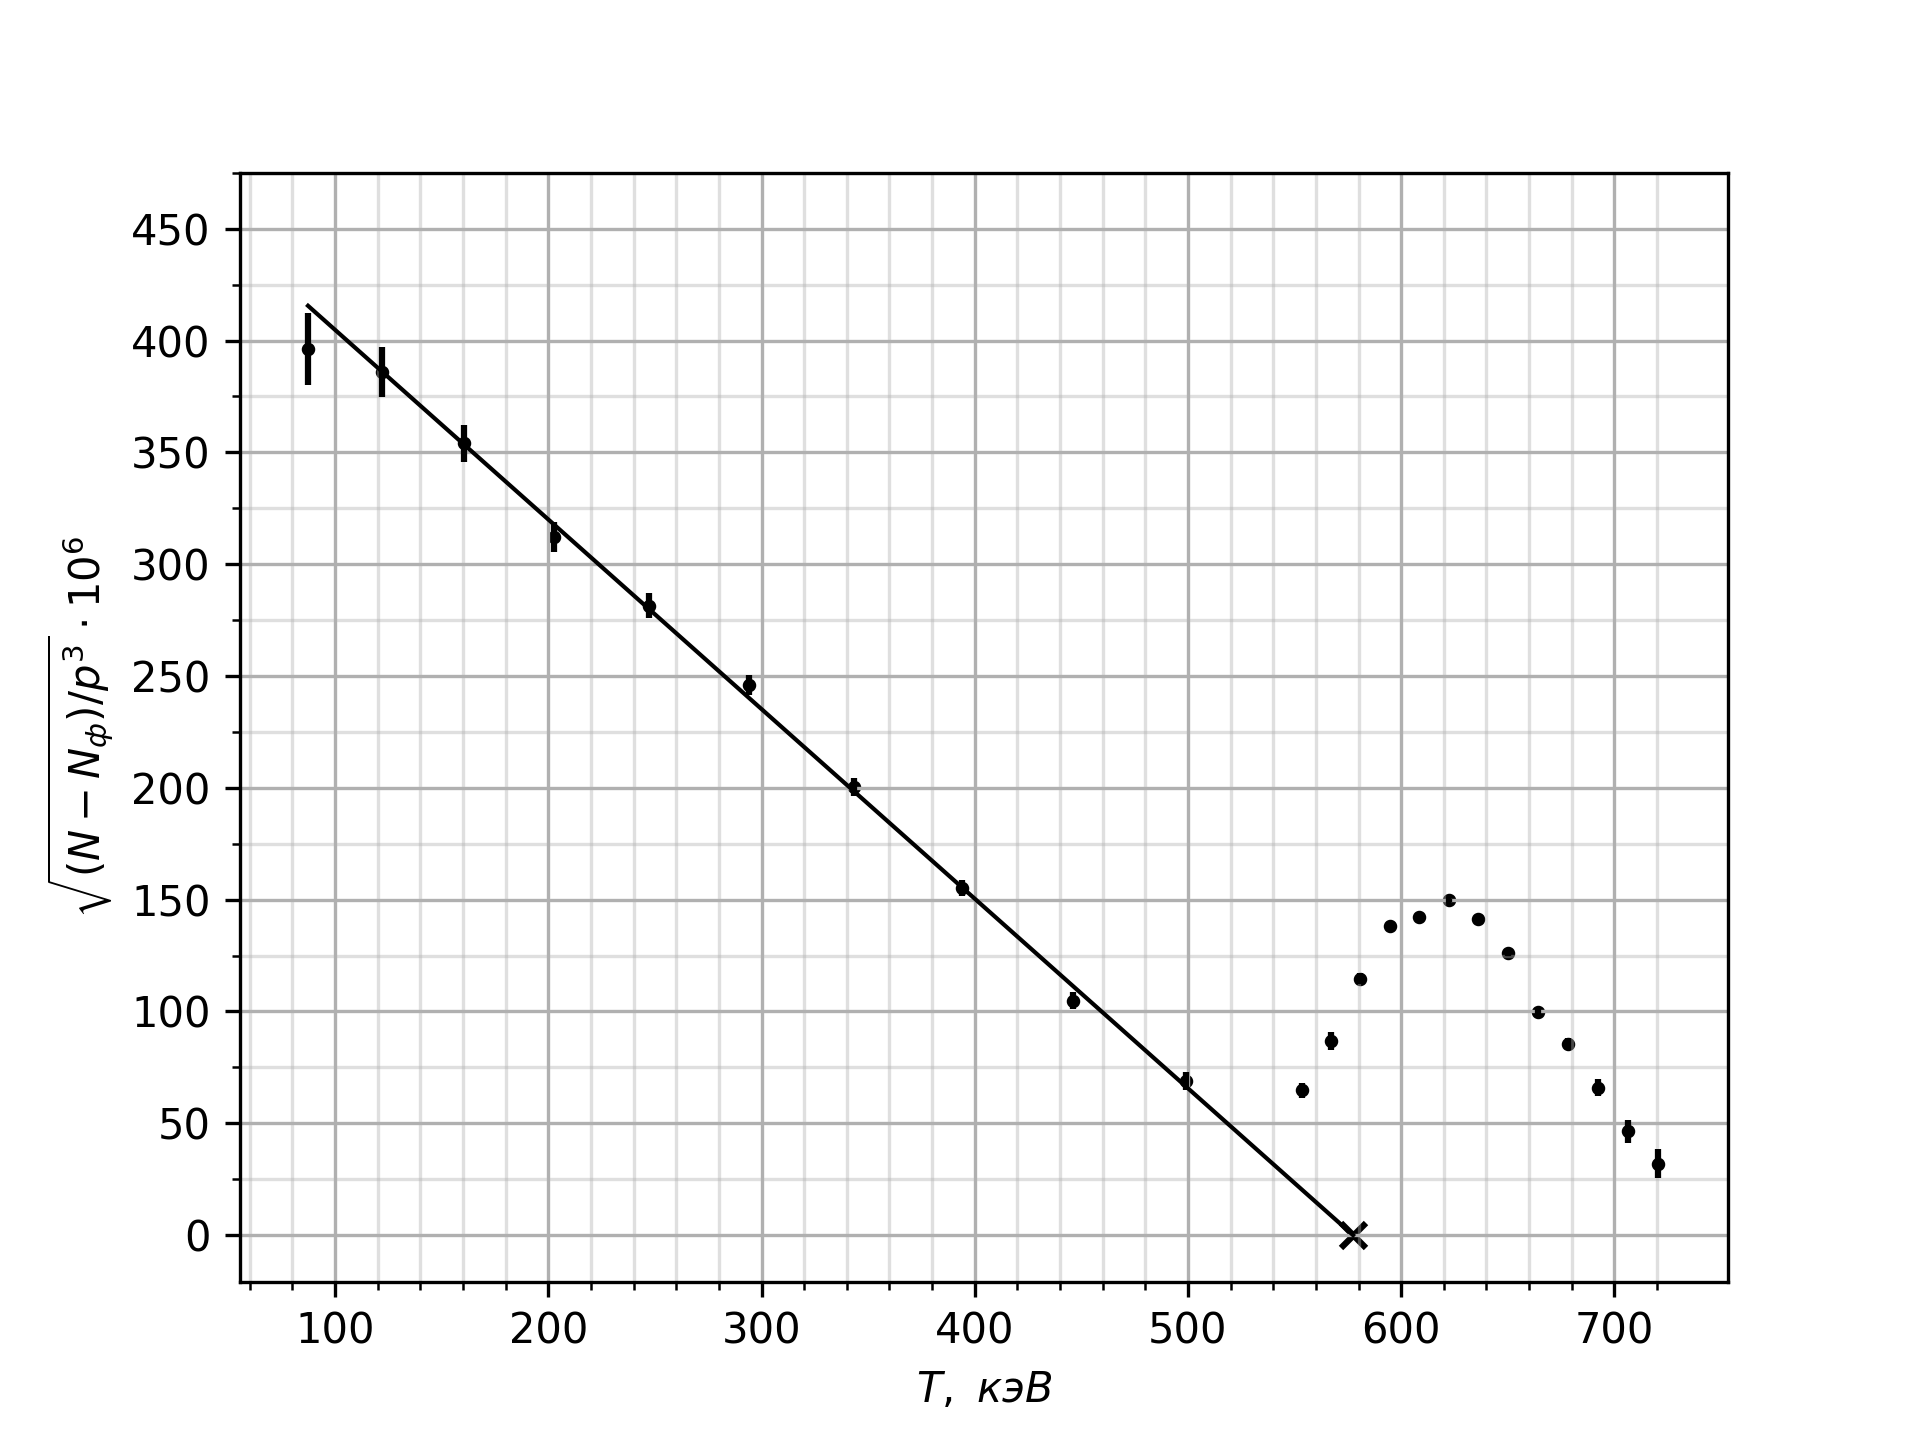
\includegraphics[scale=0.7]{../images/542-3}}
\caption{График Ферми}
\end{figure}

\item Через часть этих точек можно провести прямую. Точка пересечения этой прямой с осью абсцисс будет равна $T_{max}$:

\[T_{max}=(577\pm4)\ кэВ\]

\end{enumerate}

\section{Выводы}

В ходе работы была произведена калибровка магнитного спектрометра и определена максимальная кинетическая энергия электронов, испускаемые атомом цезия при $\beta$-распаде. Согласно данным из лабораторного практикума данное значение должно быть меньше энергии конверсионных электронов, однако мной был получен обратный результат. Для повышения точности исследования можно было повысить степень вакуума в установке и провести более длительные регистрации $\beta$-частиц.

\end{document}